\documentclass[12pt]{article}
%you can look for fun LaTeX packages to use here

\usepackage{amsmath}
\usepackage{amssymb}
\usepackage{fancyhdr}
\usepackage{multicol}
\usepackage{graphicx}
\usepackage{color}
\usepackage{amsthm}
\usepackage{hyperref}
\usepackage{amsrefs}
\usepackage{verbatim}
\usepackage{caption}
\usepackage{subcaption}
\usepackage{amsmath, epsfig}
\setlength{\parskip}{8pt}
\usepackage{xcolor}
\definecolor{shadecolor}{RGB}{150,150,150}
\usepackage{graphicx}
\graphicspath{ {./images/} }

\usepackage{blindtext}
\usepackage[T1]{fontenc}
\usepackage[utf8]{inputenc}

\newtheorem{theorem}{Theorem}
\newtheorem{lemma}{Lemma}
\newtheorem{corollary}{Corollary}
%\theoremstyle{Remark}
%\newtheorem{remark}
\newcommand{\abs}[1]{\left| #1\right|}
\newcommand{\Lap}[1]{\mathcal{L}\left\{#1\right\}}


\addtolength{\topmargin}{-.875in}
\addtolength{\textheight}{1.75in}

\newcommand{\solution}[1]{
\color{red}\begin{quote}Solution:\quad 
\color{black} #1
\end{quote}\color{black}
}
\newcommand{\ba}{\backslash}
\newcommand{\Ber}{\hbox{Ber}}
\newcommand{\p}[1]{\mathbb{P}\left(#1\right)}
\newcommand{\e}[1]{\mathbb{E}(#1)}
\newcommand{\Po}[1]{\hbox{Po}(#1)}
\newcommand{\var}[1]{\hbox{Var}(#1)}
\newcommand{\Z}{\mathbb{Z}}
\newcommand{\R}{\mathbb{R}}
\newcommand{\Q}{\mathbb{Q}}
\newcommand{\N}{\mathbb{N}}
\newcommand{\floor}[1]{\left\lfloor #1\right\rfloor}
\newcommand{\C}{\mathbb{C}}
\DeclareMathOperator{\Diam}{diam}
\newcommand{\diam}[1]{\Diam\left(#1\right)}

\DeclareMathOperator{\nul}{Null}
\newcommand{\Null}[1]{\nul\left(#1\right)}


\renewcommand{\vec}[1]{\mathbf{#1}}
\newcommand{\threevec}[3]{\left[\begin{array}{r} #1 \\ #2 \\ #3\end{array}\right]}

\newcommand{\fourvec}[4]{\left[\begin{array}{r} #1 \\ #2 \\ #3\\#4\end{array}\right]}

\DeclareMathOperator{\Rank}{rank}
\newcommand{\rank}[1]{\Rank\left(#1\right)}

\DeclareMathOperator{\Sp}{Span}
\renewcommand{\sp}[1]{\Sp\left\{#1\right\}}


%fun commands for fun sets
%make sure to use these in math mode
\newcommand{\Zset}{\mathbb{Z}}
\newcommand{\Rset}{\mathbb{R}}
\newcommand{\Nset}{\mathbb{N}}

%it may be helpful to make more commands for words/symbols you use often that you don't have to keep typing 

\oddsidemargin0cm
\topmargin-2cm    
\textwidth16.5cm   
\textheight23.5cm  

\newcommand{\question}[2] {\vspace{.25in} \hrule\vspace{0.5em}
\noindent{\bf #1 #2} \vspace{0.5em}
\hrule \vspace{.10in}}
\renewcommand{\part}[1] {\vspace{.10in} {\bf (#1)}}

\setlength{\parindent}{0pt}
\setlength{\parskip}{5pt plus 1pt}

\title{Power Method for SVD Approximation}
\author{Allen \& Jiachen (Amy) Liu}
\date{December 13th, 2018}
 
\begin{document}
 
\maketitle
 
\section{Introduction}
\vspace{-8pt}
\hspace{+24pt}Singular value decomposition (or SVD for short) is a matrix factorization method that dates back as far as the 19th century with the first proof of SVD for rectangular matrices devised by Carl Eckart and Gale Young in 1936$^{[4]}$. Applications of SVD can be found in many instances such as data compression, image processing, and noise reduction, in part due to the fact that SVD can be calculated for any rectangular matrix rather than just square matrices. While calculating SVD on smaller matrices is relatively easy, computing the singular value of an $n x n$ matrix is $O(n^3)$. $^{[7]}$ Unfortunately as a result, computing singular values on a significantly larger matrix such as images will be exponentially more time consuming. The rise of big data has caused data sets for applications in machine learning to be equally as massive and improvements in image sensor technology have pushed the boundary of photo resolution. As one can see, calculating SVD for practical uses today is often simply too inefficient.

\hspace{+24pt}As a result of this dilemma, the majority of applications of SVD today don't actually find the singular value decomposition, but rather generates the SVD using close approximations of the singular values. The Power Method is one such method. Originally devised as a way to approximate eigenvalues, we are able to use it to approximate singular values by exploiting the relationship between the two. Depending on the implementation, the Power Method's time complexity varies based on specifications. However, even in the worst case scenario, calculating the singular value using the Power Method is only $O(n^2)$,  which significantly cuts down on the computation of singular value while still producing very similar results.$^{[4]}$
 
\section{Definitions}
\vspace{-8pt}
\subsection{Limits}
\vspace{-8pt}
A limit is the value that a function (or sequence) approaches as the input approaches some value. Denoted as $\lim_{x \to c} f(x) = L$ where L is the limit.
\vspace{-8pt}
\subsection{Convergence}
\vspace{-8pt}
In the context of limits, a limit is convergent if the limit exists.
\vspace{-8pt}
\subsection{Tuple}
\vspace{-8pt}
A tuple is a finite order list (known as a sequence) of elements. If the tuple has n elements, we denote it as an n-tuple.
\vspace{-8pt}
\subsection{Dominant Eigenvalue and Eigenvector}
\vspace{-3pt}
Let $\lambda_1, \lambda_2,..., \lambda_n$ be the eigenvalues of an n x n matrix A. $\lambda_i$ is called the dominant eigenvalue of A if $|\lambda_i| > |\lambda_k|$  $\forall k \in {1,2,...,n}$ where $k \neq i$. The eigenvectors corresponding to $\lambda_i$ are called the dominant eigenvectors. $^{[5]}$

\vspace{-8pt}

\vspace{3pt}
\section{Main Theorems \& Ideas of Power Method}
\vspace{-8pt}
Recall the calculation of singular value decomposition and the definition of the eigenvalue \& eigenvector that was detailed in 21-241 Linear Algebra course. 
\vspace{-3pt}
\subsection{How \& Why the Power Method works}
\vspace{-5pt}
\hspace{24pt}The Power Method is an iterative method that approximates the dominant eigenvalue (which in the process calculates the corresponding dominant eigenvector) of a square matrix A. The reason why we can use it for SVD is that the singular values of A and $A^TA$ are the same; therefore, by taking the square root of the resulting eigenvalue of $A^TA$ from the power method, we get the singular value of A. Secondly, the eigenvector calculated from the power method is also the right singular vector. The left singular vector can be calculated through the formula $u_i = \frac{1}{\sigma_i}Av_i$ where $u_i$ is the corresponding left singular vector, $\sigma_i$ is the singular value, A is the matrix, and $v_i$ is the right singular vector.

\hspace{24pt}The power method approximates the dominant eigenvector by utilizing the fact that it is equal to $\lim_{k \to \infty} (ATA)^kx$ (see section on Convergence of Power Method below). Instead of calculating the limit, a reasonably large k is enough to give a good approximation of the dominant eigenvector. Once we have this eigenvector, we must find the corresponding eigenvalue to get the singular value. This can be achieved through the usage of Rayleigh Quotient (see section on Rayleigh Quotient below).

\hspace{24pt}To find subsequent singular values and vectors, we take the original matrix A and subtract it by $\sigma_i u_i v_i$ and run the power method on the resultant matrix. Intuitively, this works because $\sigma_i u_i v_i$ produces the best rank i approximation of the matrix A. By removing this from the matrix A can be thought of "removing" this dimension. As a result, the power method will find the next dominant eigenvector and value, producing the next best rank i+1 approximation.

\vspace{-5pt}
\subsection{Rayleigh Quotient}
If x is an eigenvector of a matrix A, then its corresponding eigenvalue is given by $$\lambda = \dfrac{Ax \cdot x}{x \cdot x}$$ As shown in class, the singular values of a rectangular matrix A is the same as the square root of the eigenvalues of $A^TA$. As a result, the Rayleigh Quotient allows one to calculate the corresponding singular value after the approximation of the right singular vector.$^{[5]}$,

\vspace{-5pt}
\subsection{Convergence of Power Method}
If A is an n x n diagonalizable matrix with a dominant eigenvalue, then there exists a nonzero vector $x_0$ such that the sequence of vectors given by
$$Ax_0, A^2x_0, A^2x_0, A^3x_0,...,  A^kx_0$$
approaches a multiple of the dominant eigenvector of A.$^{[5]}$

The proof of this theorem is shown in Elementary Linear Algebra $^{[5]}$ on page 591.

\vspace{3pt}
\section{Implementation}
\vspace{-8pt}
This section will explain the details of the cycle that finds the singular value, left singular vector, and right singular vector for the largest singular value, and repeats for the 2nd, 3rd, etc singular values and its corresponding L/R vectors. The complete set up of the entire function other than the cycle portion (such as variable naming, storage etc.) can be found on the submitted code. 

\vspace{-8pt}
\subsection{Constructing $A^TA$}
\vspace{-13pt}
\begin{align*}
    \mbox{Constructs a copy of input matrix as it is:  } & \colorbox{gray!30}{Acopy = copy.deepcopy(A)}\\
    \mbox{Computes ATA:  } & \colorbox{gray!30}{ATA = np.transpose(Acopy).dot(Acopy)}
\end{align*}
\vspace{-8pt}\\
The variable ATA represents $A^TA$. Since we need to preserve the input matrix $A$ for the future operation of subtracting the best rank approximation from $A$, we perform a deepcopy. As a part of the $copy$ package, the function returns a pointer to a another distinct numpy array that contains the same values as $A$ (in contrast to simply using $=$ that would return an alias, a pointer pointing to the original $A$ to execute calculation upon). In the 2nd line of code,  \colorbox{gray!30}{np.transpose(Acopy)} finds the $A$'s transpose, and  \colorbox{gray!30}{.dot(Acopy)} multiplies the transpose with its original, yielding $A^TA$.

\vspace{-8pt}
\subsection{Finding eigenvalue \& eigenvector}
\vspace{-8pt}
\begin{align*}
    \mbox{We choose a random vector x:  } & \colorbox{gray!30}{\textnormal{v = np.random.rand(ATA.shape[1])}}\\
     \mbox{Algorithm of sec 3.3:  } & \colorbox{gray!30}{\textnormal{for \_ in range(k):  }}\\ 
    \mbox{Matrix-vector multiplication:  } & \textnormal{~~~~~~~~}\colorbox{gray!30}{\textnormal{temp = np.dot(ATA, v)}}\\ 
    \mbox{Normalizes the vector each time:  } & \textnormal{~~~~~~~~} \colorbox{gray!30}{\textnormal{v = temp / np.linalg.norm(temp)}}\\
    \mbox{Calculate eigenvalue:  } & \colorbox{gray!30}{sval = math.sqrt(np.dot(ATA, v).dot(v) / np.dot(v,v))}\\
\end{align*}
As detailed by the main theorem's section 3.3 where the $A^kx$ for a reasonably high $k$ will yield a multiple of the dominant eigenvector, this code simulates that by initializing a random vector $v$ and conduct $v = Av$ over and over again for $k$ times as a for loop. 

On the 5th line, the eigenvalue can be calculated through a simple process. First, we calculate the dot product of $A^TA\cdot v$. We then calculate the dot product of $(A^TA \cdot v) \cdot v$. By dividing by the $||v||^2$ which can be attained by the dot product of $v\cdot v$, we get the eigenvalue. This is known as Rayleigh Quotient outlined in section 3.2. Since we that the eigenvalue is the singular value squared, we will take the square root, hence \colorbox{gray!30}{sval = math.sqrt(...)}.

\vspace{-8pt}
\subsection{Finding left singular vector}
\vspace{-8pt}
\begin{align*}
    \mbox{The left singular vector:  } & \colorbox{gray!30}{\textnormal{u = (1/sval)*A.dot(v)}}
\end{align*}
Recall from the 21-241 course, that the left singular vector, $u_i$ is obtained by $u_i = \frac{1}{\sigma_i}\cdot A\cdot v_i$ where $A$ is the original matrix and $v$ is the right singular vector.
    
\vspace{-8pt}
\subsection{Iteration}
\vspace{-8pt}
\begin{align*}
    \mbox{new $A$:  } & \colorbox{gray!30}{\textnormal{ A = A - sval*(np.dot(u.reshape(5,1),(np.transpose(v).reshape(1,10))))}}
\end{align*}
Recall that the best rank 1 approximation can be formed $A_1 = \sigma_1 u_1 v_1$. As detailed in section 3.1, by subtracting this approximation from A, we result in a $A'$ that shifts all dimensions downwards by one rank, stripped of the previously approximated singular values and L/R vectors. Thus, yielding a matrix to perform best rank 1 approximation on again. 

\section{Results}
\subsection{Provided Test Case}
\vspace{+15pt}
\[
\text{Input: } M=
  \begin{bmatrix}
    0.041 & 0.815 & 0.245 & 0.054 & 0.249 & 0.534 & 0.753 & 0.307 & 0.877 & 0.429 \\
    0.918 & 0.846 & 0.249 & 0.262 & 0.133 & 0.32 & 0.446 & 0.122 & 0.164 & 0.711 \\
    0.139 &  0.701 &  0.726 & 0.094 & 0.036 & 0.695 & 0.325 & 0.29 & 0.373 & 0.692 \\
    0.644 &  0.067 &  0.032 &  0.896 &  0.047 & 0.55 & 0.062 & 0.568 & 0.204 & 0.275 \\
    0.63 & 0.412 & 0.232 & 0.415 & 0.335 & 0.508 & 0.393 & 0.549 & 0.076 & 0.698
    
  \end{bmatrix}
\]
\vspace{+15pt}\\
The results of calling our power\_method compared to an official singular value decomposition provided by Numpy $^{[7]}$ are shown on the next page.

\begin{figure}[h!]
    \caption{Power Method Implementation Output}
    \centering
    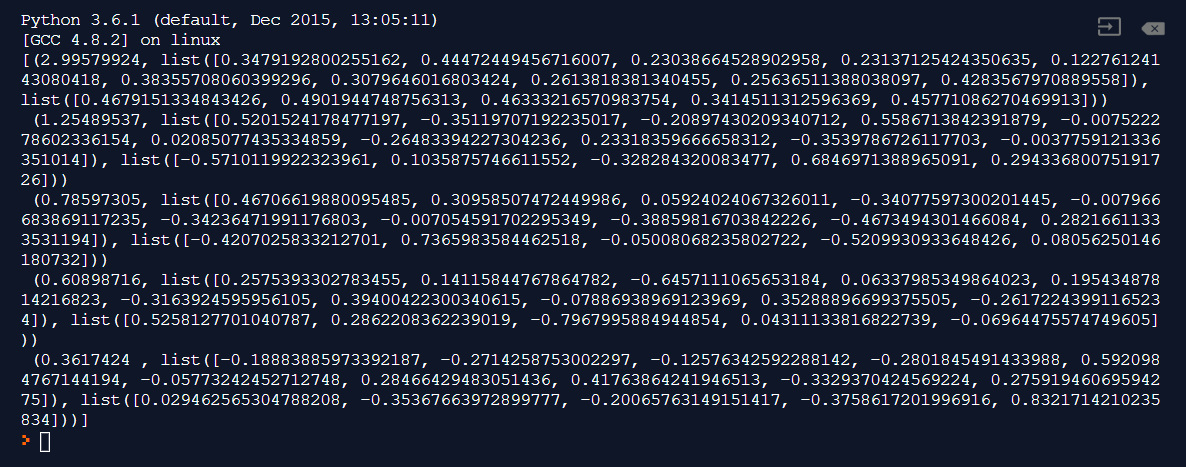
\includegraphics[scale=0.65]{pm1}
\end{figure}

\begin{figure}[h!]
    \caption{Numpy SVD Output}
    \centering
    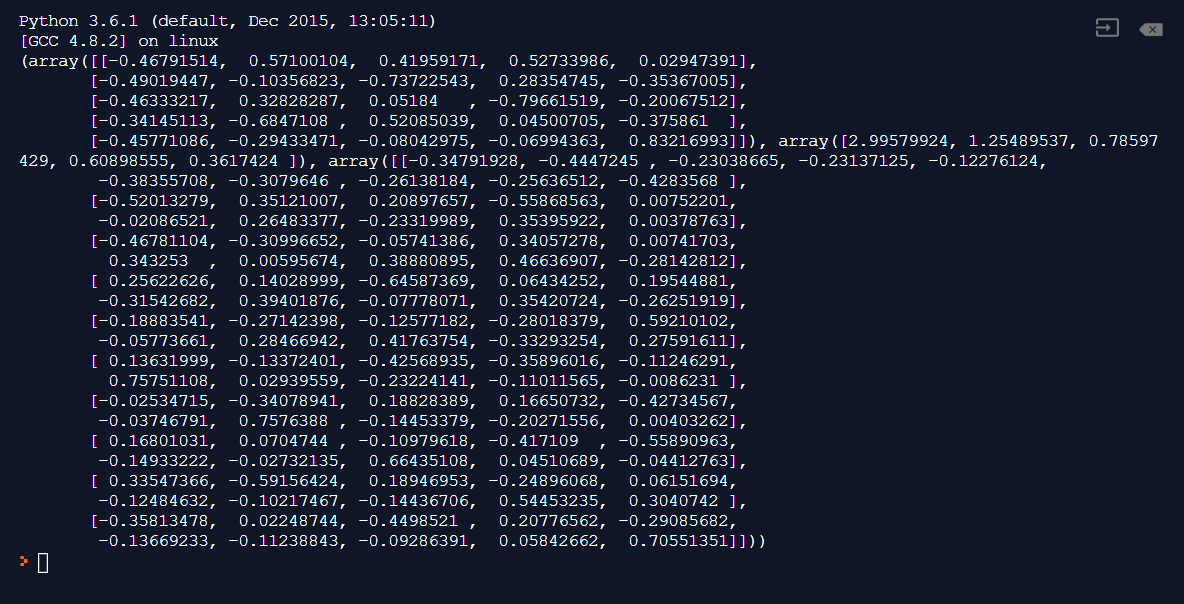
\includegraphics[scale=0.65]{svd1}
\end{figure}

\newpage

\subsection{Analysis}
\vspace{-6pt}
\hspace{+24pt} As the outputs have shown, even with a relatively small k-value of 10, the results of our power method implementation are identical to Numpy's SVD implementation up to the 7th decimal place. Depending on the application, you could get away with even lower k-values in lower precision environments.

\hspace{24pt}However, one notable difference between the two results is the sign in the first array element representing the first left and right singular vectors. Upon further research into this issue, we realized that many of today's current algorithms to find SVD (including Numpy's implementation, MATLAB, etc.) does not yield useful data from their signs. The signs of the result are simply byproducts from the numerical calculations to get the result and not actually meaningful in describing the original matrix$^{[3]}$. There is an algorithm in giving meaning to the signs from SVD created by Sandia National Laboratories; however, for the purpose of this assignment, we deemed it was not necessary to do so because of the added computational complexity required.
\vspace{-8pt}
\section{Conclusion}
\vspace{-10pt}
\hspace{+24pt}Mathematically, the power method performs its job in approximating the largest singular values and its corresponding left \& right singular vectors. For reasonably high power value, we can calculate it with an appropriate error range but at a provably lower time-complexity cost. This is an acceptable time and precision trade-off for a majority of professional fields.

\hspace{+24pt}Our code successfully simulates the Power Method algorithm with the help of python's Numpy package that performs matrix-vector multiplication and transposition. The procedure repeated appropriately to find all singular values \& L/R vectors for a full singular value decomposition. The program is capable of calculating such decomposition within fractions of a second as shown in our results section.

\hspace{+24pt}This project has shown that the power method is provenly useful and can be easily implemented for as few as a dozen lines of code. It presents a cost-efficient solution that provides comparable results to the large scale singular value decomposition that may be nearly impossible given current computational power. This is why virtually all implementation of SVD utilizes some variation of the power method to easily generate the desired values such as Google PageRank and Gumgum's natural language processing system. 

\section{Bibliography}
\begin{bibdiv}
\begin{biblist}
\bib{Blum18}{book}{
title={Foundations of Data Science},
author={Blum, Avrim},
author={Hopcroft, John},
author={Kannan, Ravindran},
date={2018-01-4},
pages={51--54},
publisher={Cornell CS},
address={Ithaca},
}

\bib{Liberty13}{misc}{
title={Lecture 7: Singular Value Decomposition},
author={Liberty, Edo},
date={Fall 2013},
organization={Yale University: 0368-3248-01-Algorithms in Data Mining},
type={Lecture notes}
}

\bib{sandia07}{report}{
title={Resolving the Sign Ambiguity in the
Singular Value Decomposition},
author={Bro, Rasmus},
author={Acar, Evrim},
author={Kolda, Tamara},
organization={Sandia National Laboratories and United States Department of Energy},
date={2007-10},
publisher={Sandia},
address={New Mexico and California},
number={SAND2007-6422}
}

\bib{Young36}{article}{
title={The Approximation of One Matrix By Another of Lower Rank},
author={Eckart, Carl},
author={Young, Gale},
journal={Psychometrika},
publisher={University of Chicago},
address={Chicago},
volume={vol.1},
number={3},
date={1936-09},
pages={211--218}
}

\bib{Larson08}{book}{
title={Elemantary Linear Algebra},
author={Larson, Ron},
author={Edwards, Bruce H.},
author={Falvo, David C.},
publisher={Houghhton Mifflin},
address={Boston},
edition={6},
date={2008-1-1},
isbn={9780618783762}
}

\bib{numpy}{webpage}{
author={The Scipy community},
date={2018-08-23},
accessdate={2018-12-14},
title={NumPy v1.15 Manual},
url={https://docs.scipy.org/doc/numpy-1.15.1/index.html},
note={Specifically, the numpy.array, numpy.linalg sections}
}


\bib{numpy}{misc}{
author={Mary Radcliffe},
date={2018-11-19},
title={Math 241: Final Project Options},
subtitle={Power Method},
note={Cited for its claim that SVD has a complexity of $O(n^3)$}
}

\end{biblist}
\end{bibdiv}
 
\end{document}